La diffusione dei dispositivi \emph{smartphone} e l'accesso ad Internet in mobilità sono ormai un dato di fatto nel panorama delle telecomunicazioni. La base di utenza si è allargata a dismisura, coprendo quasi tutte le fasce d'età così come l'infrastruttura tecnologica consente ormai di utilizzare questi mezzi in svariate situazioni permettendo di restare sempre connessi. 

L'utilizzo della applicazioni mobili è ormai parte delle nostre attività quotidiane, sia ricreative che in ambito lavorativo. Le esigenze e le sfide per questo tipo di strumenti sono sempre più ambiziose: vogliamo applicazioni \emph{smart}, che ci rendano facili e accessibili le informazioni più complesse e che offrano un'esperienza d'uso personalizzata e tagliata su misura sulle nostre richieste.

Il progetto \emph{PathS} si sviluppa in questo contesto, proponendo un'evoluzione dei sistemi di navigazione pedonale. L'idea di fondo è che la  proposta del tragitto più breve verso una destinazione non sia più l'unica informazione da fornire agli utenti, ma grazie ai recenti sviluppi tecnologici può essere integrata con un'insieme di elementi di contorno che possono rendere più coinvolgente e mirata l'esperienza di utilizzo.

Lo scopo che si è voluto raggiungere è quello di un sistema prototipale che consentisse di sperimentare questo tipo di soluzione in tutte le sue parti: l'analisi delle informazioni ambientali tramite un dispositivo \emph{smartphone}, la relativa elaborazione ed intersezione con i dati geografici, fino alla proposta di un servizio effettivo di calcolo dei percorsi che consideri criteri alternativi. Per raggiungere l'obiettivo è quindi richiesto lo studio e lo sviluppo di due elementi architetturali: la parte \emph{client mobile} che si occupa di interagire con l'utente finale e di svolgere le funzioni di misurazione tramite i sensori \emph{hardware} e la componente \emph{server} che invece gestisce l'elaborazione delle informazioni ricevute e le modella al fine di ricavarne un significato. Uno schema ad alto livello del funzionamento previsto è presentato in figura \ref{fig:paths-general}.

\begin{figure}[ht]
  \centering
  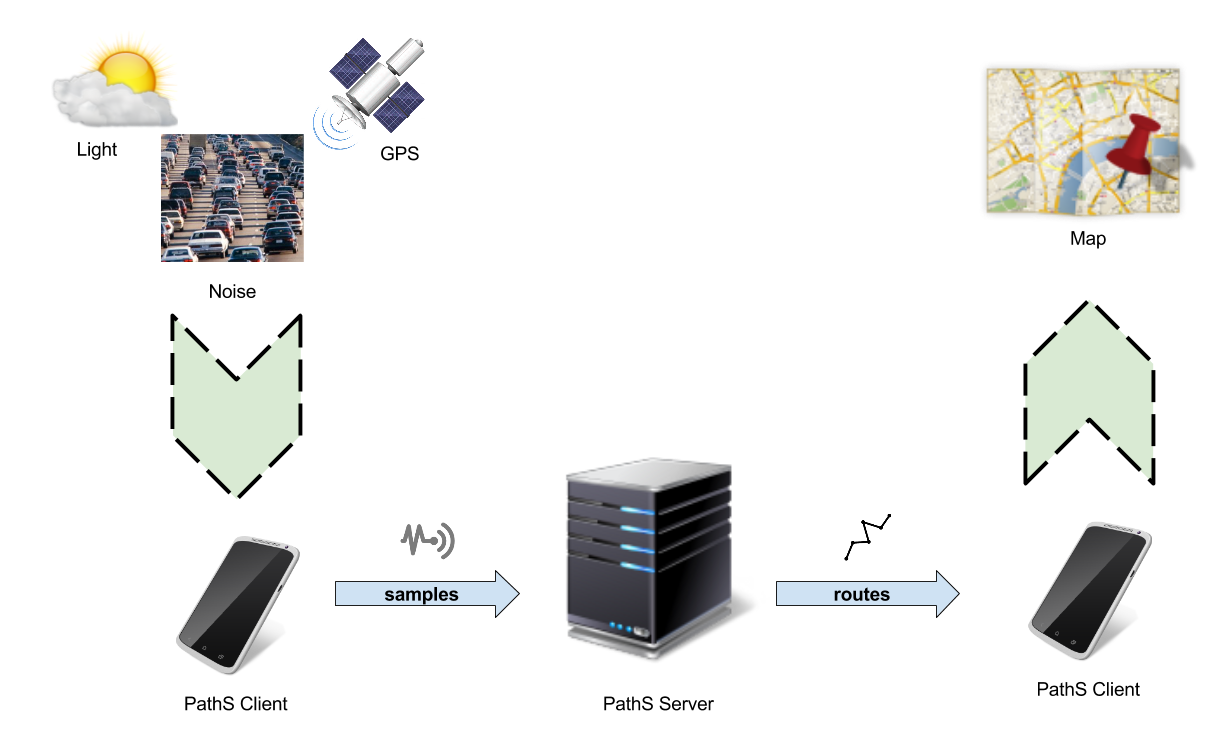
\includegraphics[width=\textwidth]{paths-general}
  \caption{\footnotesize{Schema generale del progetto PathS.}}
  \label{fig:paths-general}
\end{figure}

Le attività presentate in questa tesi riguardano principalmente gli aspetti relativi allo sviluppo del \emph{server} e le problematiche ad esso connesse. Una delle prime esigenze è stata quella di definire formalmente un protocollo di comunicazione tra le due componenti per mezzo di una API chiara e precisa, ma che al tempo stesso lasciasse la possibilità di migliorare o estendere le funzioni del software in futuro. In questa fase di sviluppo del progetto si è stabilito che gli aspetti ambientali che l'applicazione avrebbe considerato sarebbero stati la luminosità e la rumorosità.

Il passo successivo che si è affrontato è stato la selezione di un servizio di cartografia che consentisse l'accesso alle informazioni geografiche di strade e percorsi pedonali in un forma idonea all'elaborazione e persistenza in un sistema indipendente. Sono state analizzate diverse alternative fino ad identificare l'opzione idonea a supportare gli sviluppi seguenti.

La tematica affrontata successivamente è stata quella dell'elaborazione dei campioni ricevuti e la relativa associazione con le informazioni cartografiche. Una soluzione identificata per trattare questo problema è stata l'applicazione di un algoritmo di \emph{Map Matching} che si è quindi deciso di implementare seguendo una proposta selezionata tra quelle disponibili in letteratura.

Per ottenere il risultato finale la componente che restava da implementare riguardava il servizio di \emph{routing} ovvero il calcolo effettivo del percorso tenendo conto non solo degli aspetti geografici come la distanza, ma anche il dominio dei dati aggiuntivi raccolti. In termini di implementazione si è adottato un algoritmo di base fornito da una libreria e configurato opportunamente per ottenere il comportamento desiderato.

Il progetto è stato coordinato nelle attività dal Prof. Claudio Palazzi e dalla Prof.ssa Ombretta Gaggi dell'Università desgli Studi di Padova. Nelle attività di analisi e approfondimento hanno collaborato i dottorandi Matteo Ciman e Armir Bujari, mentre le attività riguardanti l'applicazione \emph{client} sono state svolte dallo studente Stefano Tombolini.

L'articolo di \textcite{web2palazzi} è stato fondamentale per l'introduzione al contesto \emph{Web\textsuperscript{2}} e alle problematiche tipiche di questo paradigma, nonchè ha fornito consigli per un approccio idoneo alla raccolta e manipolazione delle informazioni.
Altri riferimenti bibliografici importanti utilizzati durante lo studio e lo svolgimento del progetto sono stati: il testo \textit{Mobility Data Management and Exploration} di \textcite{mdme} per quanto concerne l'approccio alla gestione dei dati generati da oggetti in movimento e l'articolo di presentazione dell'algoritmo \emph{ST-Matching} come riferimento per l'implementazione.

In questo elaborato saranno presentati inizialmente il contesto e un insieme di progetti che per problematica affrontata o approccio utilizzato risultano affini e di interesse. Saranno introdotti alcuni elementi di letteratura in particolare riguardo la tematica dei \emph{Mobility Data}.

Il capitolo \ref{cap:client} fornirà un riassunto delle caratteristiche e delle funzioni offerte della componente \emph{client}, le quali risultano fondamentali per una visione complessiva del progetto.

I capitoli successivi documentano le attività di analisi e implementazione del \emph{server PathS} nelle sue macro-funzioni: ricezione, analisi dei campioni e calcolo dei percorsi pedonali.

L'ultimo capitolo fornirà un esempio dei risultati raggiunti e proporrà alcune aree di miglioramento così come sono state individuate durante lo svolgimento delle attività.
